%! Author = Philipp Emmenegger
%! Date = 09/06/2021

\section{Reviews}
\textbf{What to review:}
\begin{itemize}
    \item Requirements
    \item Architecture
    \item Design
    \item Usability
    \item Code
    \item Product
    \item Process
    \item Progress
    \item Collaboration
\end{itemize}
\textbf{Principles}
\begin{itemize}
    \item Timely
    \item Systematic
    \item Reasonable
\end{itemize}

\subsection{Techniques}
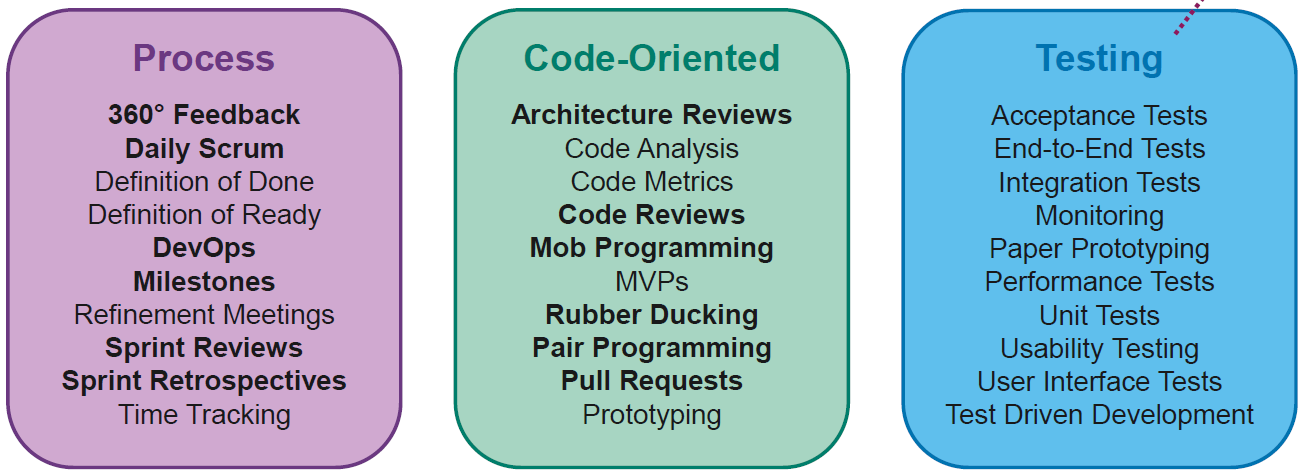
\includegraphics[width=\linewidth]{../img/review_techniques.png}

\subsubsection{Sprint Review}
\begin{itemize}
    \item ca. 1h per week
    \item Maybe start with presentation (state of project / goals / backlog / metrics)
    \item Involve the audience
    \item Attending the review should be fun
\end{itemize}

\subsubsection{Sprint Retrospective}
\begin{itemize}
    \item Communicate usefulness early and often
    \item Send invitations early / regularly
    \item Prepare materials in the room
    \item Repeat the rules before the meeting
    \item Findings should have impact on upcoming iterations
    \item Early in the project, go for quick wins
    \item Keep open impediments in a backlog
    \item Communicate progress
\end{itemize}
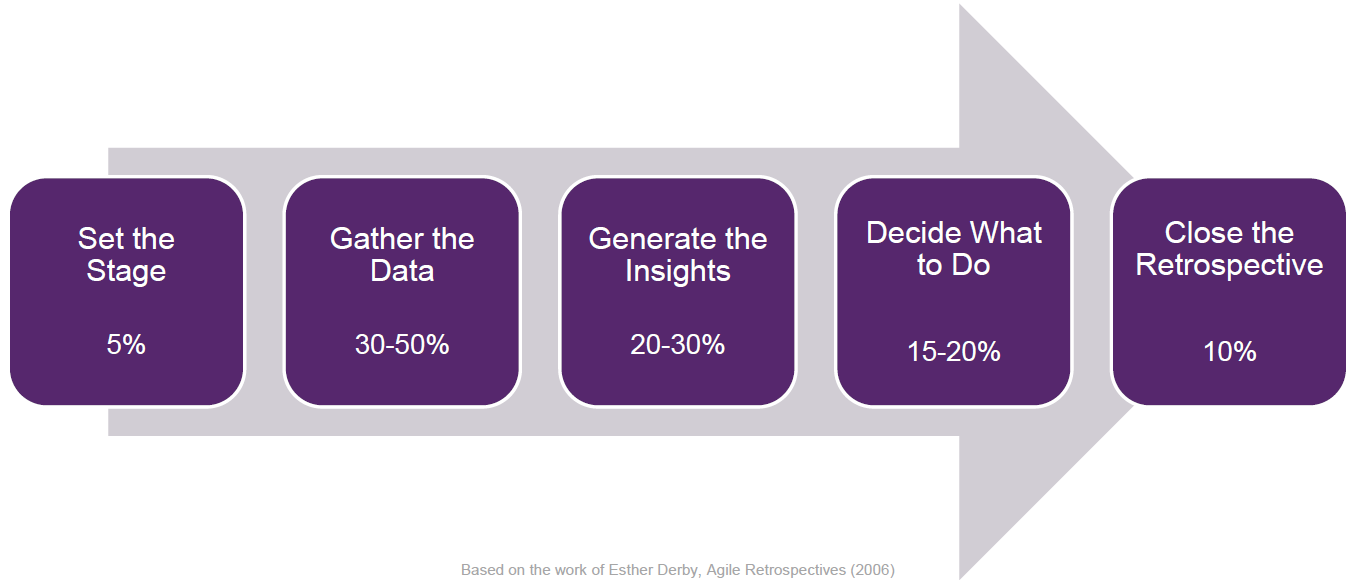
\includegraphics[width=\linewidth]{../img/sprint_retrospective.png}

\subsubsection{DevOps}
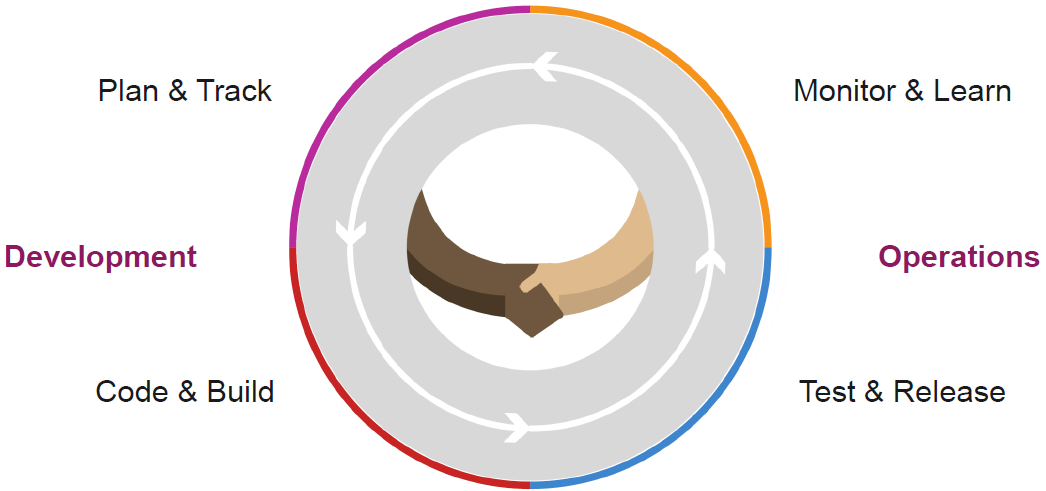
\includegraphics[width=0.7\linewidth]{../img/devops.png}

\subsubsection{360deg Feedback}
\begin{itemize}
    \item Incorporate results from different sources
    \item Self-assessment
    \item Manager
    \item Collaborators
    \item Customers
    \item Only works in an environment of trust
\end{itemize}

\subsection{Code-oriented Techniques}
\subsubsection{Rubber Ducking}
\textit{siehe clean coder oder so..}

\subsubsection{Pair Programming}
\textit{siehe clean coder oder so..}

\subsubsection{Mob Programming}
\begin{itemize}
    \item Pair programming with more attendees (Devs, Architects, Domain Experts...)
    \item Best suited for very difficult problems / mission critical parts of code
\end{itemize}

\subsubsection{Pull Requests}
\begin{enumerate}
    \item Dev makes changes on a branch
    \item Dev files a pull request
    \item Rest of the team reviews the code (check DoD)
    \item Maintainer merges into a stable branch
\end{enumerate}

\subsubsection{Code Reviews}
\begin{itemize}
    \item Formal way to assess code
    \item Performed manually, supported by tools
    \item Use it deliberately
\end{itemize}
\textbf{Roles}
\begin{itemize}
    \item Author
    \item Reviewer
    \item Moderator
    \item Recorder
    \item Attendee
\end{itemize}
\textbf{Artifacts}
\begin{itemize}
    \item Protocol
    \item Work Items (optional)
\end{itemize}
\textbf{Process:}
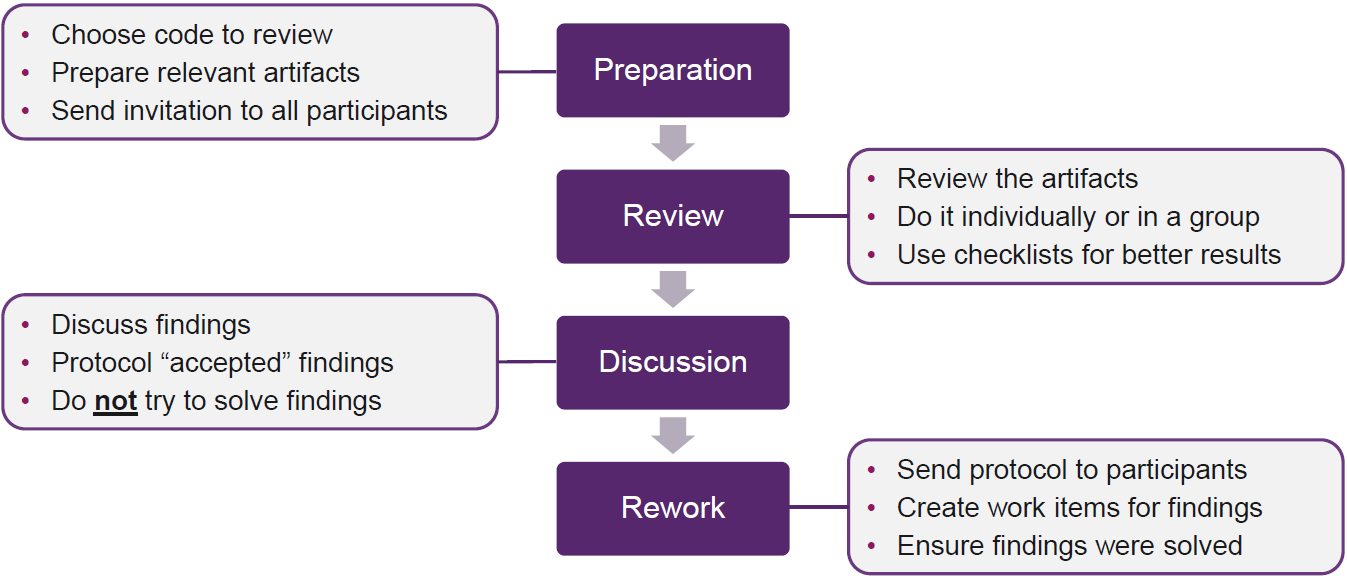
\includegraphics[width=\linewidth]{../img/code_reviews_process.png}
\textbf{Dos:}
\begin{itemize}
    \item Respect Feedback rules
    \item Only review code that satisfies DoD
    \item Choose appropriate amount of code
    \item As a reviewer, take your time
    \item Support the review with automated tools
    \item Use checklists
    \item Highlight positive examples
\end{itemize}
\textbf{Don'ts}
\begin{itemize}
    \item Fixing code during the review
    \item Never review simple code
    \item Do not invite people responsible for the author
\end{itemize}

\subsection{Architecture Reviews}
\begin{itemize}
    \item Quantitative: Metrics and Profiling
    \item Qualitative: Reviews ATAM
    \item combine the both!
\end{itemize}

\subsubsection{ATAM - Architecture Tradeoff Analysis Method}
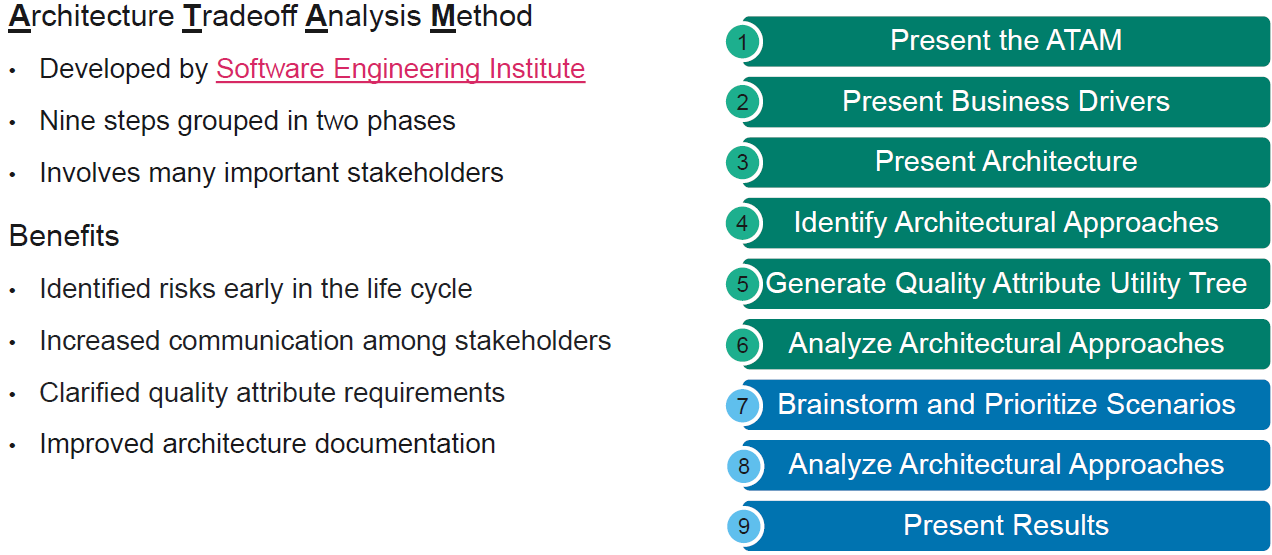
\includegraphics[width=\linewidth]{../img/ATAM.png}
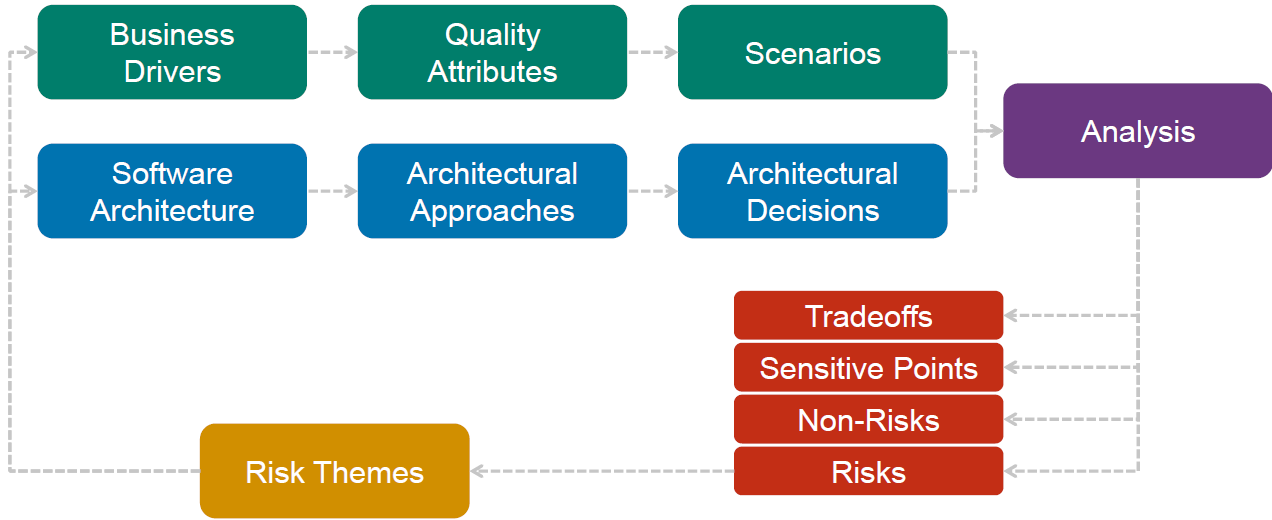
\includegraphics[width=\linewidth]{../img/ATAM_flow.png}

